\input{header.tex}
\input{newcommands.tex}


\title{Anki-Karteikarten, Multiple-Choice-Tests und QTI aus einer Liste}
\author{Fortbildungsmaterial für Lehrkräfte}
\date{\today}
\pagestyle{plain}
\setlength{\parskip}{1.5em} % Abstand zwischen Absätzen (Handreichungen)
\setlength{\emergencystretch}{4em} % lange \texttt-Wörter umbrechen statt über den Rand


\begin{document}

\maketitle

Anki ist ein kostenloses Karteikartenprogramm, das jede Karte genau dann wieder abfragt, wenn man sie zu vergessen droht (verteiltes Wiederholen). Es läuft am Computer, auf Android (AnkiDroid) und auf iPhone und iPad (AnkiMobile). Karten von Hand anzulegen ist mühsam. Das Python-Skript \texttt{anki\_karten.py} baut aus einer einfachen Liste einen fertigen Stapel (\texttt{.apkg}): Doppelklick, und die Karten sind in Anki. Aus derselben Liste mit Multiple-Choice-Fragen entstehen außerdem ein Papiertest mit Lösungsteil und ein QTI-Paket für Testsysteme wie ONYX.

\tableofcontents



%%%%  KAPITEL 1  %%%%
\section{Einrichten}

Benötigt werden Python ab Version~3.11 und das Paket \texttt{genanki}, für den Papiertest außerdem \hologo{LaTeX}:

\begin{lstlisting}[style=latex]
pip install genanki
\end{lstlisting}

\begin{center}
\begin{tabular}{@{}>{\raggedright\arraybackslash}p{4.6cm}>{\raggedright\arraybackslash}p{3.4cm}>{\raggedright\arraybackslash}p{6.8cm}@{}}
	\toprule
	\textbf{Du änderst} & \textbf{Werkzeug} & \textbf{Ergebnis} \\
	\midrule
	CSV (Vokabeln, Begriffe, Formeln) oder Textdatei (Multiple Choice) & \texttt{anki\_karten.py} & \texttt{.apkg} für Anki; bei Multiple Choice zusätzlich Test als \texttt{.tex} und QTI-Paket \\
	\bottomrule
\end{tabular}
\end{center}



%%%%  KAPITEL 2  %%%%
\section{Vokabeln, Begriffe und Formeln}


%%%%  UNTERKAPITEL 2.1  %%%%
\subsection{Die Liste}

Eine CSV-Datei mit den Spalten \texttt{Vorderseite;Rückseite;Zusatz;Tags}. Trennzeichen dürfen Semikolon, Komma oder Tabulator sein; \texttt{Zusatz} und \texttt{Tags} sind optional. Die erste Zeile ist die Überschrift:

\begin{lstlisting}[style=latex]
Englisch;Deutsch;Zusatz;Tags
to achieve;erreichen, schaffen;She achieved her goal.;verb
reliable;zuverlässig;a reliable source;adjektiv
to apply for sth.;sich für etw. bewerben;to apply for a job;verb
\end{lstlisting}

\begin{lstlisting}[style=latex]
python3 anki_karten.py vokabeln englisch_beispiel.csv --deck "Englisch::Unit 3" --rueckrichtung
\end{lstlisting}

\texttt{-{}-deck} ist der Name des Stapels; mit \texttt{::} entstehen Unterstapel. \texttt{-{}-rueckrichtung} fragt beide Richtungen ab (Englisch $\to$ Deutsch und Deutsch $\to$ Englisch), \texttt{-{}-anzahl 20} nimmt nur 20 zufällige Einträge.


%%%%  UNTERKAPITEL 2.2  %%%%
\subsection{Formeln}

Formeln stehen wie in \hologo{LaTeX} zwischen Dollarzeichen und werden in Anki mit MathJax gesetzt:

\begin{lstlisting}[style=latex]
Vorderseite;Rückseite;Zusatz;Tags
Ableitung von $x^n$;$n\cdot x^{n-1}$;Potenzregel;ableitung
Ableitung von $\sin x$;$\cos x$;;ableitung
\end{lstlisting}

\begin{lstlisting}[style=latex]
python3 anki_karten.py vokabeln mathe_formeln.csv --deck "Mathematik::Formeln"
\end{lstlisting}


%%%%  UNTERKAPITEL 2.3  %%%%
\subsection{Bilder}

Bilder bindet man mit \texttt{[bild:dateiname.png]} ein; die Dateien liegen in dem Ordner, den \texttt{-{}-bilder} angibt. Das Beispiel fragt die Bundesländer ab. Die 16 Bilder sind mit der Vorlage \texttt{vorlage\_bundeslaender\_bilder.tex} aus den Karten des Skills \texttt{latex-geodaten-karten} entstanden:

\begin{lstlisting}[style=latex]
Vorderseite;Rückseite;Zusatz;Tags
Welches Bundesland ist markiert? [bild:sh.png];Schleswig-Holstein;Landeshauptstadt: Kiel;geografie
Welches Bundesland ist markiert? [bild:hh.png];Hamburg;Landeshauptstadt: Hamburg (Stadtstaat);geografie
\end{lstlisting}

\begin{lstlisting}[style=latex]
python3 anki_karten.py vokabeln bundeslaender.csv --deck "Geografie::Bundesländer" --bilder bilder
\end{lstlisting}

So sehen die Karten in Anki aus, links eine Bildkarte, rechts eine Formelkarte:

\begin{ausgabe}
	\centering
	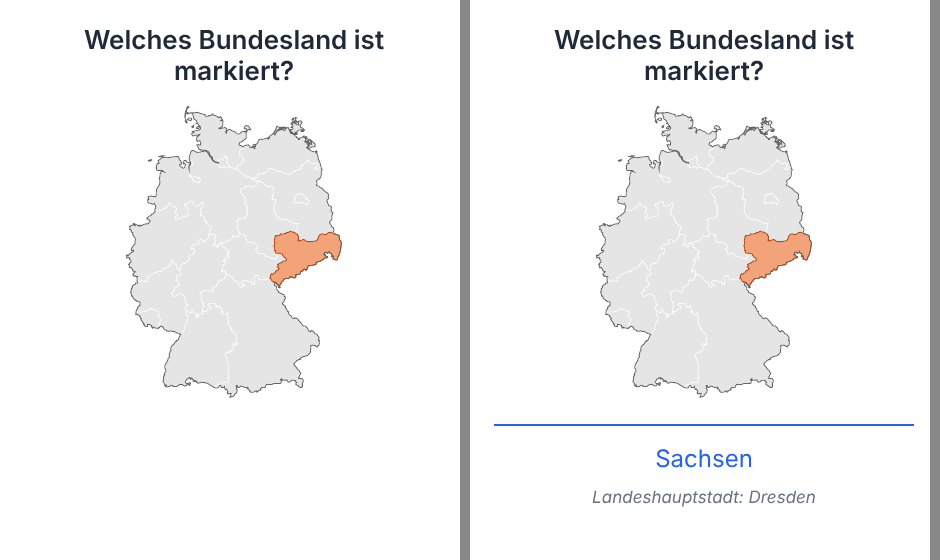
\includegraphics[width=0.48\linewidth]{anki_bild.png}\hfill
	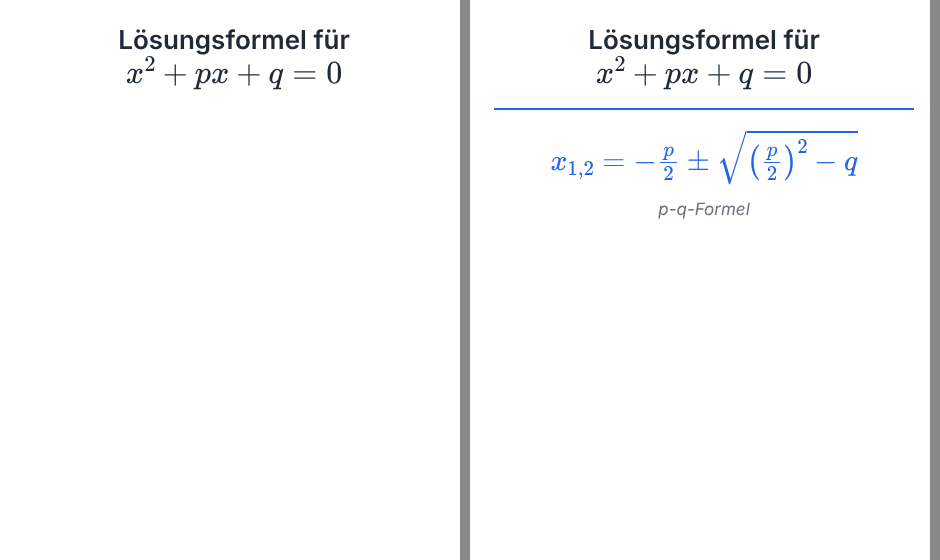
\includegraphics[width=0.48\linewidth]{anki_formel.png}
\end{ausgabe}

\begin{merke}
	Importiert man eine geänderte Liste erneut, werden die vorhandenen Karten \textbf{aktualisiert} statt doppelt angelegt; der Lernfortschritt bleibt erhalten. Erkannt wird eine Karte an ihrer Vorderseite. Ändert man die Vorderseite, entsteht deshalb eine neue Karte.
\end{merke}



%%%%  KAPITEL 3  %%%%
\section{Multiple Choice}


%%%%  UNTERKAPITEL 3.1  %%%%
\subsection{Das Format}

Für Multiple-Choice-Fragen, etwa zum Training für die Besondere Leistungsfeststellung (BLF) oder das Abitur, gibt es ein eigenes Textformat. Jede Frage ist ein Block, Leerzeilen trennen die Fragen:

\begin{lstlisting}[style=latex]
? Gegeben ist $f(x) = -(x-1)^2 + 4$. Welche Aussagen sind wahr?
+ Der Scheitelpunkt ist $S(1 \mid 4)$.
+ Die Parabel ist nach unten geöffnet.
+ Die Nullstellen sind $x_1 = -1$ und $x_2 = 3$.
- Der Graph schneidet die $y$-Achse im Punkt $(0 \mid 4)$.
> $f(0) = -1 + 4 = 3$, also Schnittpunkt $(0 \mid 3)$.
@ quadratische_funktionen
\end{lstlisting}

\begin{center}
\begin{tabular}{@{}cl@{}}
	\toprule
	\textbf{Zeichen} & \textbf{Bedeutung} \\
	\midrule
	\texttt{?} & Frage (Folgezeilen ohne Zeichen gehören zur Frage) \\
	\texttt{+} & richtige Antwort; mehrere \texttt{+} ergeben eine Mehrfachauswahl \\
	\texttt{-} & falsche Antwort \\
	\texttt{>} & Erklärung auf der Rückseite (optional) \\
	\texttt{@} & Tags (optional) \\
	\texttt{\%} & Kommentarzeile \\
	\bottomrule
\end{tabular}
\end{center}

In Anki erscheinen die Antworten mit Buchstaben; auf der Rückseite sind die richtigen markiert, darunter steht die Erklärung:

\begin{ausgabe}
	\centering
	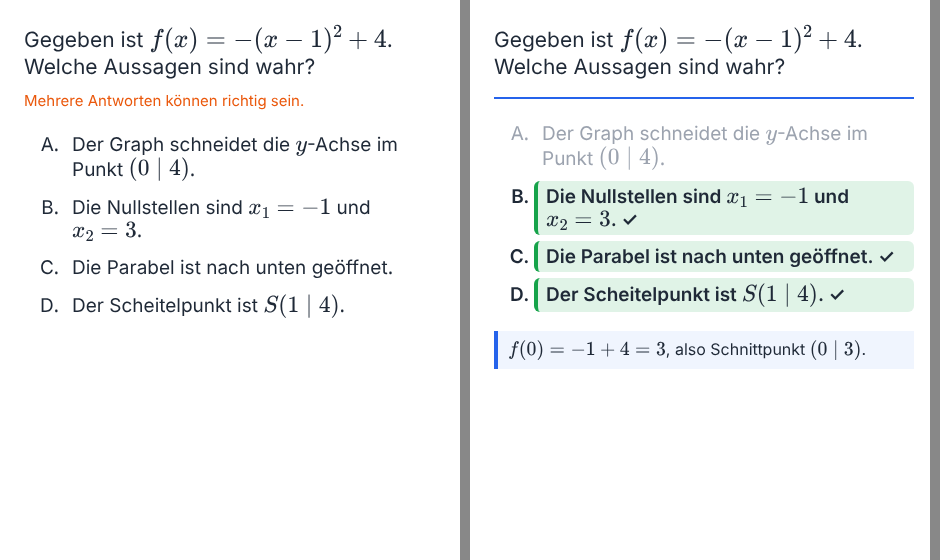
\includegraphics[width=0.8\linewidth]{anki_mc.png}
\end{ausgabe}


%%%%  UNTERKAPITEL 3.2  %%%%
\subsection{Stapel, Papiertest und QTI aus einer Datei}

\begin{lstlisting}[style=latex]
python3 anki_karten.py mc fragen_blf_mathe.txt --deck "Mathematik::BLF-Training" --mischen --pdf --qti --titel "BLF-Training Mathematik – Multiple Choice"
pdflatex fragen_blf_mathe.tex
\end{lstlisting}

\texttt{-{}-mischen} mischt die Antwortreihenfolge einmalig, \texttt{-{}-pdf} schreibt zusätzlich einen Test als \texttt{.tex} mit Lösungsteil, \texttt{-{}-qti} ein QTI-2.1-Paket (\texttt{.zip}) für Testsysteme. Der Papiertest aus den zehn Beispielfragen:

\begin{ausgabe}
	\centering
	\fbox{\includegraphics[page=1, width=0.47\linewidth]{fragen_blf_mathe.pdf}}\hfill
	\fbox{\includegraphics[page=3, width=0.47\linewidth]{fragen_blf_mathe.pdf}}
\end{ausgabe}

\begin{hinweis}[Noch ungetestet]
	Der QTI-Import in ONYX ist noch nicht ausprobiert. Formeln kommen dort als \hologo{LaTeX}-Text an, Bilder werden nicht übernommen. Laut ONYX-Hilfe geht auch ein CSV-Import; die Beispiel-CSV dafür gibt es in ONYX selbst. Damit lässt sich das Skript passend erweitern.
\end{hinweis}



%%%%  KAPITEL 4  %%%%
\section{Fragen mit einer KI erstellen}

\begin{hinweis}[Beispiel-Prompt]
	\itshape Erstelle 25 Multiple-Choice-Fragen zur Vorbereitung auf die BLF Mathematik (Sachsen) im Format von fragen\_blf\_mathe.txt: je vier Antworten, plausible Falschantworten aus typischen Fehlern, kurze Erklärung mit >, Tags nach Themengebiet, Formeln in \$\dots\$, Dezimalkomma als \{,\}.
\end{hinweis}

Fragen und Antworten einer KI muss man fachlich prüfen, bevor sie in den Stapel kommen. Personenbezogene Daten gehören nicht in den Prompt.



%%%%  KAPITEL 5  %%%%
\section{Alle Optionen}

\begin{center}
\begin{tabular}{@{}l>{\raggedright\arraybackslash}p{11cm}@{}}
	\toprule
	\textbf{Option} & \textbf{Bedeutung} \\
	\midrule
	\texttt{vokabeln} / \texttt{mc} & Art der Eingabe: CSV-Liste oder Multiple-Choice-Textdatei \\
	\texttt{-{}-deck} & Name des Stapels, Unterstapel mit \texttt{::} (Pflicht) \\
	\texttt{-{}-ausgabe} & Name der \texttt{.apkg} (Standard: wie die Eingabedatei) \\
	\texttt{-{}-bilder} & Ordner mit den Bildern für \texttt{[bild:\dots]} \\
	\texttt{-{}-tags} & Tags für alle Karten \\
	\texttt{-{}-rueckrichtung} & zusätzlich Rückseite $\to$ Vorderseite abfragen \\
	\texttt{-{}-anzahl}, \texttt{-{}-seed} & nur so viele zufällige Einträge; \texttt{seed} macht die Auswahl wiederholbar \\
	\texttt{-{}-mischen} & Multiple Choice: Antwortreihenfolge einmalig mischen \\
	\texttt{-{}-pdf}, \texttt{-{}-titel} & Multiple Choice: Papiertest als \texttt{.tex} mit Überschrift \\
	\texttt{-{}-qti} & Multiple Choice: QTI-2.1-Paket für Testsysteme \\
	\bottomrule
\end{tabular}
\end{center}



%%%%  KAPITEL 6  %%%%
\section{Zusammenfassung}

\begin{itemize}
	\item Liste schreiben (CSV oder Multiple-Choice-Textdatei), \texttt{anki\_karten.py} starten, \texttt{.apkg} doppelklicken.
	\item Formeln in \texttt{\$\dots\$}, Bilder mit \texttt{[bild:\dots]} und \texttt{-{}-bilder}.
	\item Erneuter Import aktualisiert die Karten und erhält den Lernfortschritt.
	\item Aus Multiple-Choice-Fragen entstehen Stapel, Papiertest und QTI-Paket aus einer Datei.
\end{itemize}

Quellen: genanki, \url{https://github.com/kerrickstaley/genanki}; Anki-Handbuch, \url{https://docs.ankiweb.net}; IMS QTI 2.1, \url{https://www.imsglobal.org/question/qtiv2p1/imsqti_infov2p1.html}.

\end{document}
